\subsection{\mfname Modeling Overview}
\label{sec:model}

A \mfname model is specified by a the following three components: 
\begin{enumerate*}[label=(\roman*)]
	\item a plant that has a collection of cells where each cell can perform certain operations;
	\item  a set of widgets that move  through the cells and each widget is associated with a requirement that defines the sequence of operations that need to be performed on the widget for it to be complete; and
	\item a controller that orchestrates  the operations at cells and movement of widgets.
\end{enumerate*}
Next we formally describe each of these parts and in Section~\ref{sec:dts_def} we define the transition system model of the entire system that is defined by these three components.

 	
\subsection{Plant Description}
The plant models the floor plan of the factory, the layout of cells and the connections between them. There is a set $\OP$ of operations and the plant model specifies what cell can perform which of these operations on widgets. 
In addition, there are two special operation corresponding to creation ($\optop$) and removal ($\opbot$) of widgets. 
We define $\OPALL = \OP \cup \{\optop,\opbot\}$.


Formally, a  {\em plant\/} is specified by a tuple $P $ $=$ $\langle G_P, \Lmap_P{}, \Tmap_P{}, \Qmap_P{} \rangle$, 
    where 
    \begin{enumerate*}[label=(\roman*)]
      \item $G_P = \langle V_P,E_P \rangle$  is a graph of cells, where $V_P$ is the set of cells; the set of edges $E_P$ define the paths for moving widgets in the floor; 
%      \item $\OP$ is a set of (possible) operations;  
      \item $\Lmap_P{}: V_P \mapsto 2^{\OPALL}$ maps each cell to the set  of operations that can be performed at that cell;
      \item $\Tmap{}: V_P \times \OPALL \mapsto \mathbb{N}$ maps a cell $v \in V$ and an operation $op \in \Lmap(v)$ to a natural number $\Tmap{(v,op)}$ which is the amount of time (measured in number of transitions) needed to complete $op$ at $v$; 
      \item $\Qmap{}: V_P \mapsto \mathbb{N}$ maps each cell to its queue length $\Qmap{(v)}$, which is the maximum number of widgets that can be queued at $v$.
    \end{enumerate*}
For any graph and $G_P$ in particular, for any vertex $v \in V_P$
 $\next(v)$ and $\prev(v)$ denote the set of predecessors and successors of $v$ in $G_P$. 
 
\paragraph*{Sources and Sinks}
 A {\em source \/} is a cell $v \in V$ such that $\optop \in \Lmap{(v)}$ and $\prev(v) = \emptyset$.
A  {\em sink\/} is a cell $v$ with $\opbot \in \Lmap{(v)}$ and $\next(v) = \emptyset$.  
 For simplicity, in this paper we assume that there is a single source ($\verttop$) and a single sink ($\vertbot$)  in any plant $P$ and 
 that $ \Lmap{(\verttop)} = \{\optop\}$ and $\Lmap{(\vertbot)} = \{\opbot\}$. 
A cell in $V$ that is neither a source nor a sink is an {\em ordinary\/} cell. 

%\cy{CY: Should we mention that $\Tmap{v,op}$ is infinite (or zero?) if $op$ is not in $L_v$? (This is for some widgets to bypass a cell.)}
%\sayan{Yes, we may need this.}
	

\subsection{Widgets and Requirements}
For modeling convenience, we assume that there exists a universal set  $W$ of unique identifiers for {\em all} widgets that will ever be seen by the manufacturing system.
% 
This includes the actual widgets in the system, those that have been finished and those that are yet to start. We denote by $\Wtop$ the set of widgets that have not been created, that is, $W_\top = \{w \in W \ | \ \loc(w) = \verttop \}$. Similarly, $\Wbot$ is the set of widgets at the sink, and  $\Word = W \setminus (\Wtop \cup \Wbot)$.
For all the results presented in the paper, a sliding window of unique identifiers would be adequate. 
A possible implementation of this will be by attaching a unique RFID tag for each widget \cite{huang2008rfid}. 

A \emph{requirement models} the sequence of operations in $\OP$ that need to be performed on each widget for the widget to be completed. Formally, a requirement is specified by a directed acyclic graph (DAG) $R = \langle V_R, E_R \rangle$ and a labeling function $L_R:V_R\rightarrow {\OPALL}$.  Further, we require that there is a single vertex $v\ \in V_R$ with no incoming edges; this vertex is called the source of $R$ and $L_R(v) = \optop$. Finally, vertices with  no outgoing edges are called sinks, and every such vertex $v$ has $L_R(v) = \opbot$.
A {\em path\/} of $R$ is a sequence of vertices in $V_R$, $\pi = v_0,\ldots,v_k$ such that $v_0$ is the source, $v_k$ is a sink, and $(v_i,v_{i+1})\in E_R$ for each $i$ in the sequence. Given a path $\pi$, we define $L_R(\pi) =  L_R(v_0),\ldots,L_R(v_k)$ which is the corresponding sequence of operations in ${\OPALL}$.


\begin{example}
\label{ex:simple_plant}
%\sayan{Show a simple layout in figure. Define the corresponding graph and parameters also in Figure. This will be a running example throughout this section of the paper.}
Consider a manufacturing system consisting of three cells $V=\{v_1, v_2, v_3\} \cup \{\verttop, \vertbot\}$.
The plant can be represented as a graph $G=(V,E)$ shown as the graph below.
The circles in the graph are cells while black squares represent conveyors.
Then the operations that supported by a cell $v$ can be obtained by $L(v)$. For example, $L(v_3)=\{op_2,op_3\}$.
Let's further consider two widget types being fabricated in this plant.
Assuming requirement 1 requires to complete $op_1$ and $op_2$ and requirement 2 requires to complete $op_1$ and $op_3$ in the given order, then the requirements are denoted by $R_1=\{op_1 \ra op_2\}$ and $R_2=\{op_1 \ra op_3\}$, $\mathcal{R}=\{R_1, R_2\}$.

\begin{figure}[ht]
	\begin{center}
		\resizebox{0.3\textwidth}{!}{%
		    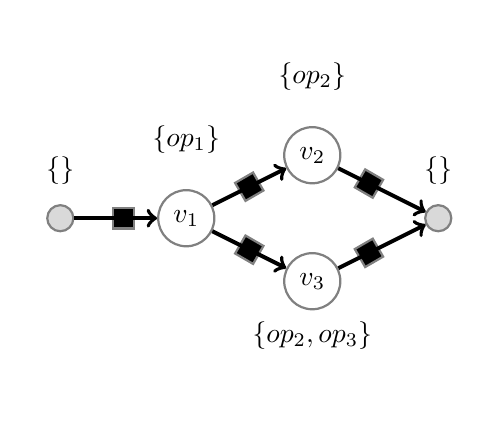
\begin{tikzpicture}
	    		%[scale=.8,auto=left,every node/.style={circle,fill=blue!20}]
	            [scale=0.8,auto=left,every node/.style={circle,draw=black!50, thick}, every path/.style={line width=0.5mm}]
	            
				\node[circle, fill=gray!30, label={$\{\optop\}$}] (v_o) at (-3,0) {$\verttop$};
	            \node[label={$\{op_1\}$}] (v_1) at (-1,0) {$v_1$};
				\node[label={$\{op_2\}$}] (v_2) at (1,1) {$v_2$};
				\node[label={[xshift=0cm, yshift=-2cm]\{$op_2,op_3\}$}] (v_3) at (1,-1) {$v_3$};
				\node[circle, fill=gray!30, label={$\{\opbot\}$}] (v_u) at (3,0) {$\vertbot$};
				
				\node[rectangle, fill=black, minimum size=7.5pt] (c_1) at (-2, 0) {};
				\node[rectangle, fill=black, minimum size=7.5pt, rotate=30] (c_2) at (0, 0.5) {};
				\node[rectangle, fill=black, minimum size=7.5pt, rotate=60] (c_3) at (0, -0.5) {};
				\node[rectangle, fill=black, minimum size=7.5pt, rotate=60] (c_4) at (1.9, 0.55) {};
				\node[rectangle, fill=black, minimum size=7.5pt, rotate=30] (c_5) at (1.9, -0.55) {};
				
				\path (v_o) edge[->] (v_1);
				\path (v_1) edge[->] (v_2);
				\path (v_1) edge[->] (v_3);
				\path (v_2) edge[->] (v_u);
	            \path (v_3) edge[->] (v_u);
		   \end{tikzpicture}
		}
	\end{center}
    \vspace{-0.25cm}
	\caption{The plant graph of a simple example.}
	\label{fig:exmaple_graph}
\end{figure}

\end{example}

\subsection{Concepts related to plants and requirements}
% Presenting these as concepts and later we say who computes what.
%In this section, we present several definitions that will be used throughout this paper.
%\sayan{Skipping this section for now. Feasible graphs/paths will probably come after introduction of controller.}
 
%Given a requirement $R = \langle O_R, E_R \rangle$ a $\mi{feasible graph}$ of a requirement $R$ is a subgraph of $G_P$ such that all paths in the $F_r$ satisfy all the paths in $R$. For a path in $F_r$ to satisfy a path in $R$, all the operations along a path in $R$ must be able to be completed by the cells along a path in $F_r$ in the same order. Note that this does not preclude a path from $F_r$ having cells which don't correspond to any node in $R$.

%Formally, a $\mi{feasible graph}, F_r = \langle V_r, E_r \rangle$ is a subgraph of $G_p$ where $V_r, E_r$ are subsets of $V_p, E_r$ respectively, Each path in $F_r$ begins at a $\mi{source}$ of the plant and terminates at a $\mi{sink}$. 
    
%\subsection{Additional Notation}
%This is a list of notation used in the plant/controller variables/transitions along with their explanations.
% Tree/Node operations
 
% Queue operations
Each $\queue(v)$ has the following operations: $\head$, returns the element at the front of the queue; $\len$, provides the current length of the queue up to a maximum specified by $\Qmap(v)$; and $\pop$, removes and returns the element at the head of the queue and decrements the $\len$ by one. 
% Additional notation
Additionally, we define the following notation: $\bag(v) := \{ w \mid \loc(w) = v\}$; $\Bag := \cup_{v \in V } \bag(v)$.

\subsection{Discrete Transition System}
\label{sec:dts_def}
We now describe the nominal  plant and an abstract controller. 
Additional variables may be added to this model, for example, to implement specific  controllers strategies and to track more complex performance metrics. 

\subsubsection*{Plant Variables}
\figref{plant-variables} gives the names and types of the plant variables ($X_p$).
The  variable $\loc$ gives the  cell at which each widget is located. Initially, all widgets are at the source $\verttop$, which indicates that they have not yet been created. When a widget is consumed at a sink its location is set to $\vertbot$. 
%
The plant variable $\pos$ assigns, for each widget, $w \in \Word$ a natural number. If $\loc(w) \in V$ then $\pos \leq Q(loc(w))$ and it is the actual position of $w$ in the queue of $\loc(w)$ (otherwise, $w \notin \Word$ and $\pos(w)$ is meaningless).
%
The variable $\queue$ is the queue (array) of widgets at that cell. As specified by the plant $P$, for any cell $v \in V_P$, the length of $\queue(v)$ is upper bounded by $Q(v)$. Initially, the queue is empty (\ie all entries are set to $\bot$).
%
The variable $\req$ selects and assigns a requirement $R \in \mathcal{R}$ to a widget. The selection of $R$ will determine the set of operations that are performed on the widget. 
%
Finally, $\widgettime$ tracks the total time a widget spent in the plant starting from $\verttop$ and ending at $\vertbot$. All widgets have their $\widgettime$ initialized to 0.

\begin{figure}[!ht]
	\centering
	\mybox{\linewidth}{\linewidth}{
		\lstinputlisting[language=ioaNums,numbersep=-3pt]{Specifications/plant_vars.txt}
		\caption{\scriptsize Plant ($X_p$) variables and types.}
	\figlabel{plant-variables}
	}
\end{figure}

\subsubsection*{Abstract Controller Variables}
\figref{abstract-cell-variables} shows the list of abstract controller variables:
%The controller variable $\completed$ keeps track of the sequence of operations that have been performed on each widget. Initially, it is the empty sequence for every widget. 
The $\timer$ keeps track of the current time of the  overall system.
%
The variable $\action$ encodes the actuation decision made by the controller for each cell $v$ for the following plant transition in which the cell $v$ uses the decision to perform some operation.
%
The variable $\nexttr$ specifies for each cell $v$ a neighboring cell   to which $v$ should transfer a widget  when it receives a  $\transfer$ action controller.
%
A concrete controller uses these and other variables to make decisions and keep track of the overall system state. 

\begin{figure}[!ht]
	\centering
	\mybox{\linewidth}{\linewidth}{
		\lstinputlisting[language=ioaNums,numbersep=-3pt]{Specifications/abstract_cell_vars.txt}
		\caption{\scriptsize Abstract controller variables.}
	\figlabel{abstract-cell-variables}
	}
\end{figure}

\subsubsection*{Plant Transitions}
During each plant transition, all the cells are updated  based on the decisions made by the controller that are reflected in the controller variables such as $\action$. These variables are read by the plant.
An ordinary operation $\op \in OP$ causes the plant to perform this operation on the current widget. There are several special actions: $\move$  moves widgets on conveyors, $\optop$ creates new widgets at sources, $\opbot$ removes finished widgets at sinks and $\transfer$ moves widgets between adjacent connected cells in the plant. We now discuss these transitions in more detail.

% Move action
If a conveyor cell $v$ is provided with a $\move$ action, $v$ decrements the position of each of the widgets in $\queue(v)$.
% OP action
If a cell is given the $\OP$ action, the cell starts to perform $\op$ on the widget at the head of its queue. While this presumably changes the local physical state of the plant and the widget, in our model, this action does not change any plant variables. Instead, we will see later that once $\op$ completes then the controller will update the record for the widget. 

% Instantiate action
If a source cell $v$ is given the $\optop$ action, it selects a widget from $w' \in \Wtop = \bag(\verttop)$, the set of widgets at the source,  $\verttop$, and assigns it a requirement $R$. This nondeterministic choice models the uncertainty in the type of requirement that is demanded from the next widget. The location of the new widget $w'$ is set to be $\verttop$ and its position is set to the end of its queue.
%
% Terminate action
If a sink cell is given the $\opbot$ action, the cell will remove the widget from the head of its queue and the removed widget's location is set to  $\vertbot$.
%
% Noop action
If a cell is given a $\noop$ action, the cell does not change any of the variables.
%
% Transfer action
If a cell is given a $\transfer$ action, the cell removes the widget at the head of its queue and reads the $\nexttr$ variable to determine the next cell to transfer the removed widget. The cell transfer the widget to the next cell by changing the location of the widget to that of the next cell and the position to the end of the next cell.


% THIS IS FOR THE ABSTRACT CONTROLLER
%\subsection*{Controller Transitions}
%During each controller transition, the controller increments $\timer$ by 1 and iterates through all the cells to update their $\cost$, $\action$, and $\nexttr$ variables.

\begin{figure}[!ht]
	\centering
	\mybox{\linewidth}{\linewidth}{
		\lstinputlisting[language=ioaNums,numbersep=-3pt]{Specifications/plant_trans.txt}
		\hfill
		\caption{\scriptsize Plant ($X_p$) transitions.}
        \figlabel{plant-transitions}
        }
\end{figure}


